% ======================================================================
% Appendix A — h* observations
% ======================================================================

\appendix
\section{The \boldmath$h^*$-observations through \boldmath$n=10$}
\label{sec:hstar}

This appendix records the Ehrhart observations on the LR-zonotopes,
extended by this session to $n=9$ and $n=10$ in both core families. The
extension was executed as a one-day addendum with a narrow purpose:
establish whether the real-rootedness and log-concavity observed at
$n\le8$ continue, and whether the strictness decay and the
non-correlation with covering margins persist. Both answers are yes. The
appendix closes with the statement we regard as the residual question of
independent interest.

\subsection{The table}

Table~\ref{tab:hstar} lists, for each family and $n$: the
$h^*$-polynomial, real-rootedness (verified \emph{exactly} by
Sturm-sequence sign-change counts on the square-free part of the integer
polynomial---the earlier $45$-decimal-place numerical verification and
the companion-matrix check agreeing---upgraded in this revision from the
numerical form), log-concavity and Newton's inequalities (exact rational
arithmetic), and the minimum ratio $h_k^2/(h_{k-1}h_{k+1})$, which is
the \emph{strictness} $S$ of log-concavity, together with the Newton
floor $\bigl((k{+}1)(d{-}k{+}1)\bigr)/\bigl(k(d{-}k)\bigr)$ at the
minimizing $k$ and the excess ratio $S/\text{floor}$. Every row's Ehrhart data was
verified three ways (Eulerian expansion, standard inversion, and an
independent depth-first coset count at $t=1,2$), the volume identity
$e_{n-1}=\sum v_j$ was asserted exactly, and the loneliness identities
$\lambda=1/(n{+}1)$ (harmonic) and $\lambda=2/(2n{+}1)$ (rung-2) were
re-asserted exactly. The $n\le8$ rows reproduce the program's earlier
records digit for digit; the $n=9,10$ rows are new.

\begin{table}[htbp]
\centering
\footnotesize
\caption{$h^*$-polynomials of the LR-zonotopes, $n=3..10$, both core
families. ``RR'' = real-rooted (exact Sturm verification, this
revision; previously $45$ dps numerical); ``LC/Nw'' = log-concave and
Newton (exact rational arithmetic); $S$ =
$\min_k h_k^2/(h_{k-1}h_{k+1})$; $nS$ = $n\cdot S$;
``floor'' = the Newton bound
$\bigl((k{+}1)(d{-}k{+}1)\bigr)/\bigl(k(d{-}k)\bigr)$ at the
minimizing $k$ (any real-rooted family has $S\ge\text{floor}$ there);
$S/f$ = $S/\text{floor}$. The $n\le8$ rows reproduce the program's
earlier records digit for digit; the $n=9,10$ rows are new (this
session); the floor and ratio columns are new in this revision.}
\label{tab:hstar}
\begin{tabularx}{\textwidth}{@{} l c >{\raggedright\arraybackslash}X c c r r r r @{}}
\toprule
family & $n$ & $h^*(z)$ & RR & LC/Nw & $S$ & $nS$ & floor & $S/f$ \\
\midrule
harm. & 3 & $1+7z+4z^2$ & y & y & $12.250$ & $36.8$ & $4$ & $3.06$ \\
rung2 & 3 & $1+11z+6z^2$ & y & y & $20.167$ & $60.5$ & $4$ & $5.04$ \\
harm. & 4 & $1+18z+35z^2+6z^3$ & y & y & $9.257$ & $37.0$ & $3$ & $3.09$ \\
rung2 & 4 & $1+22z+51z^2+10z^3$ & y & y & $9.490$ & $38.0$ & $3$ & $3.16$ \\
harm. & 5 & $1+37z+179z^2+133z^3+10z^4$ & y & y & $6.511$ & $32.6$ & $9/4$ & $2.89$ \\
rung2 & 5 & $1+45z+239z^2+181z^3+14z^4$ & y & y & $7.013$ & $35.1$ & $9/4$ & $3.12$ \\
harm. & 6 & $1+78z+744z^2+1286z^3+399z^4+12z^5$ & y & y & $5.518$
& $33.1$ & $2$ & $2.76$ \\
rung2 & 6 & $1+86z+920z^2+1682z^3+535z^4+16z^5$ & y & y & $5.748$
& $34.5$ & $2$ & $2.87$ \\
harm. & 7 & $1+147z+2522z^2+8948z^3+7323z^4$\newline
$+1201z^5+18z^6$ & y & y & $4.335$ & $30.3$ & $16/9$ & $2.44$ \\
rung2 & 7 & $1+161z+3024z^2+11144z^3+9295z^4$\newline
$+1551z^5+24z^6$ & y & y & $4.418$ & $30.9$ & $16/9$ & $2.48$ \\
harm. & 8 & $1+290z+8317z^2+51458z^3+82947z^4$\newline
$+35270z^5+3135z^6+22z^7$ & y & y & $3.791$ & $30.3$ & $5/3$ & $2.27$ \\
rung2 & 8 & $1+298z+9277z^2+60986z^3+102275z^4$\newline
$+44798z^5+4095z^6+30z^7$ & y & y & $3.829$ & $30.6$ & $5/3$ & $2.30$ \\
harm. & 9 & $1+559z+25519z^2+258901z^3+734059z^4$\newline
$+631993z^5+155305z^6+8035z^7+28z^8$ & y & y & $3.293$ & $29.6$ & $25/16$ & $2.11$ \\
rung2 & 9 & $1+585z+28885z^2+305035z^3+880149z^4$\newline
$+764143z^5+188659z^6+9789z^7+34z^8$ & y & y & $3.323$ & $29.9$ & $25/16$ & $2.13$ \\
harm. & 10 & $1+1098z+77550z^2+1213626z^3+5529648z^4$\newline
$+8309694z^5+4180482z^6+626910z^7+19359z^8+32z^9$ & y & y & $2.987$
& $29.9$ & $3/2$ & $1.99$ \\
rung2 & 10 & $1+1114z+83790z^2+1377794z^3+6457600z^4$\newline
$+9866694z^5+5017826z^6+758710z^7+23631z^8+40z^9$ & y & y & $3.004$
& $30.0$ & $3/2$ & $2.00$ \\
\bottomrule
\end{tabularx}
\end{table}

The sweep families behave identically: every instance of $(1,2,m)$,
$m\le14$, and $(1,2,3,m)$, $m\le12$, tested by the program was
real-rooted, log-concave, and Newton.

\subsection{Strictness decay and non-correlation}

Two quantitative facts were already in the program's records at $n\le8$
and persist through the new rows; both are stated here with the precision
the data supports. First, the strictness $S$ decays monotonically in $n$
in both families, with $n\cdot S$ drifting from $\approx37$ at
$n=3,4$ (harmonic; the rung-2 family starts at $60.5$) to
$\approx29.6$--$30.0$ at $n=9,10$: within the measured range the decay
is well described as $\approx30/n$. That description cannot persist
indefinitely---log-concavity forces $S\ge1$, and Newton's inequalities
force $S$ above the floor $\bigl((k{+}1)(d{-}k{+}1)\bigr)/\bigl(k(d{-}k)
\bigr)\approx1+4/d$ at the middle coefficients, so $nS\approx30$ would
cross the floor near $n\approx26$---and much of the measured decline is
the generic Newton-floor decline that any real-rooted family exhibits.
The family-specific content is the excess $S/\text{floor}$, which declines
from $3.06$ (harmonic) and $5.04$ (rung-2) at $n=3$ to $1.99$ and
$2.00$ at $n=10$ (Table~\ref{tab:hstar}, Figure~\ref{fig:nS}); it, too,
declines, so there is no growing quantitative margin in the coefficient
structure to spend. Second, the strictness carries no statistically
distinguishable correlation with the covering margins at the achievable
sample sizes: across the $n=3$ sweep (twelve instances, $(1,2,m)$,
$m=3..14$) the Spearman coefficient of strictness against the margin is
$+0.32$ ($p=0.32$); across the $n=4$ sweep (eight instances,
$(1,2,3,m)$, $m=5..12$) it is $-0.31$ ($p=0.45$). The sign flips
between adjacent rungs and neither coefficient is significant; these
arrays are too small to establish correlation or its absence. The
harmonic family has margin identically $0$ at every $n$ while its
strictness varies by a factor of four over the table. Both coefficients
were recomputed in the provenance run from the persisted instance data
and reproduce exactly.

\begin{figure}[htbp]
\centering
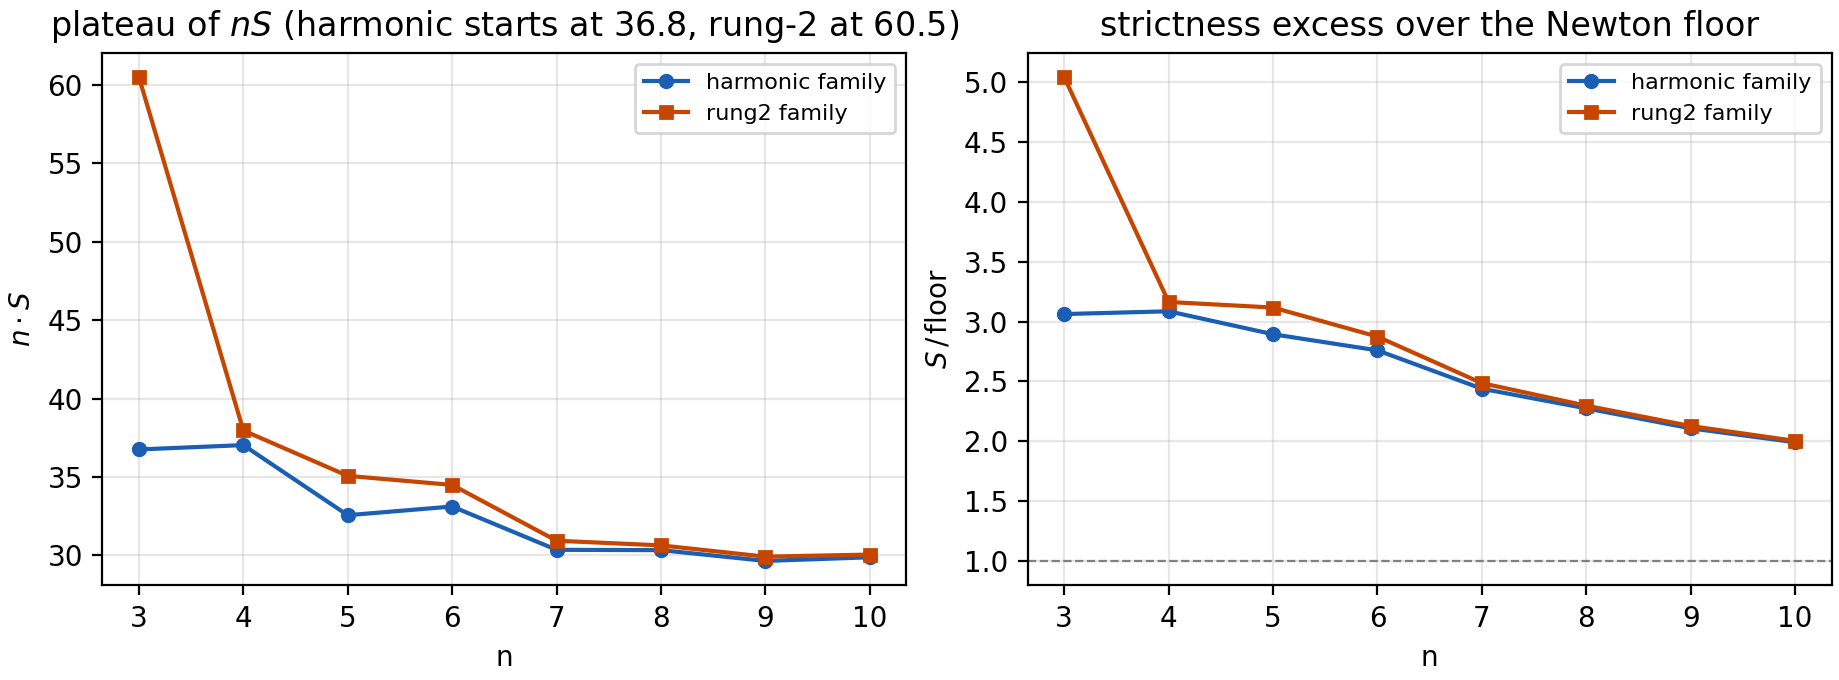
\includegraphics[width=0.92\textwidth]{fig_nS.png}
\caption{The strictness records of Table~\ref{tab:hstar}. Left: the
plateau of $n\cdot S$ (the harmonic family starts at $36.8$, rung-2 at
$60.5$; both drift to $\approx30$). Right: the excess $S/\mathrm{floor}$
over the Newton floor at the minimizing coefficient---the
family-specific content of the decline---which itself decreases from
$3.06$/$5.04$ at $n=3$ to $1.99$/$2.00$ at $n=10$.}
\label{fig:nS}
\end{figure}

The two facts close the bridge in the coefficient direction, and the
falsity of the covering-radius statement (\S\ref{sec:tm-zono}) closes it
in the metric direction: the statement that strict log-concavity would
have needed to feed is false at the extremal instances, and the
coefficient structure cannot see the metric hole depth that falsifies
it. There is no mechanism, and the arithmetic is clean enough that the
absence of the mechanism is itself a datum.

\subsection{The residual question}

What survives is a question of independent arithmetic interest, and we
state it decoupled from the Lonely Runner problem entirely. The
Ehrhart data of the LR-zonotopes is governed by the gcd structure
\eqref{eq:ehr} of the projected basis---the arithmetic matroid of the
configuration \cite{dAMoci}. In every instance tested (two core
families through $n=10$, sweeps through $m\le14$ at $n=3$ and $m\le12$
at $n=4$), the arithmetic $h^*$-polynomial is real-rooted.

\begin{conjecture}\label{conj:hstarRR}
The $h^*$-polynomial of the arithmetic matroid of any projected basis
$\pi([0,1]^n)\cap\Lambda$ of the form considered here---in particular,
for every speed vector $v=(v_1,\dots,v_n)$ with distinct entries and
$\gcd(v)=1$---is real-rooted.
\end{conjecture}

The conjecture is stated for the projected-basis zonotopes; the sweeps
suggest it may hold for $(1,\dots,n-1,m)$ and beyond, and the natural
home for it is the real-rootedness and Lorentzian literature for
arithmetic matroid Tutte specializations
\cite{BrandenHuh,dAMoci,StanleyEC}. We
flag it as a question, record the data, and deliberately do not pursue
it further here: the extension to $n=9,10$ was executed to complete the
record, and the record's reading is that the question is real but
belongs to a different subject. It is not a bridge, and treating it as
one would repeat the pattern this paper documents.
